
%\section{Overview of the Silicon Tracking System (STS)}
All semiconductor based detector systems include very similar functions. The signals from the detector channels have to be amplified and processed for storage and analysis. The silicon sensors, analog-digital converter and all the necessary support structures are often referred to as a detector module. Nevertheless, there are many parameters that have to be optimized in order to achieve the detector performance.

The use of microstrip silicon sensors was demonstrated in other experiments around the world. It's design and thickness are primarily dependent on the constraints related to the scaterring and signal over noise ratio. 

This chapter aims to present an introduction to the silicon based detector systems and general working principles. Subsequently, the design of the \gls{STS} is discussed with focus on the hardware and its control. At last, the requirements for the detector control system are considered. 

\section{Role of the semiconductors based detector}

Semiconductors can be considered as ionization chambers, which are features a pair of electrodes and applied external voltage. The particles passing through the volume of a sensor may result in forming an electron and hole pair. A typical charge deposition by a minimum ionizing particle in a \SI{300}{\micro\metre} thick wafer is around 25000 electron-hole pairs. The deposited charge is retrieved by one or more strips per side, what results in position determination. The analog signals are converted into digital ones, processed and analyzed.

In the simplest case, a plate could be used as an electrode, but it wouldn't be possible to determine the position of a particle very precisely. To address this problem, the electrodes can be segmented into strips. Figure~\ref{fig_si} shows an example of implementing segmented electrodes to determine the particle position. In order to achieve the two-dimensional information, the second electrode has usually an inclination of a few degrees. Apart from microstrip sensors, there are also for example pixel devices which enable determining two-dimensional positions. It can be achieved either by proper segmentation of the electronics or designing the geometry.  

\begin{figure}[!h]
\centering
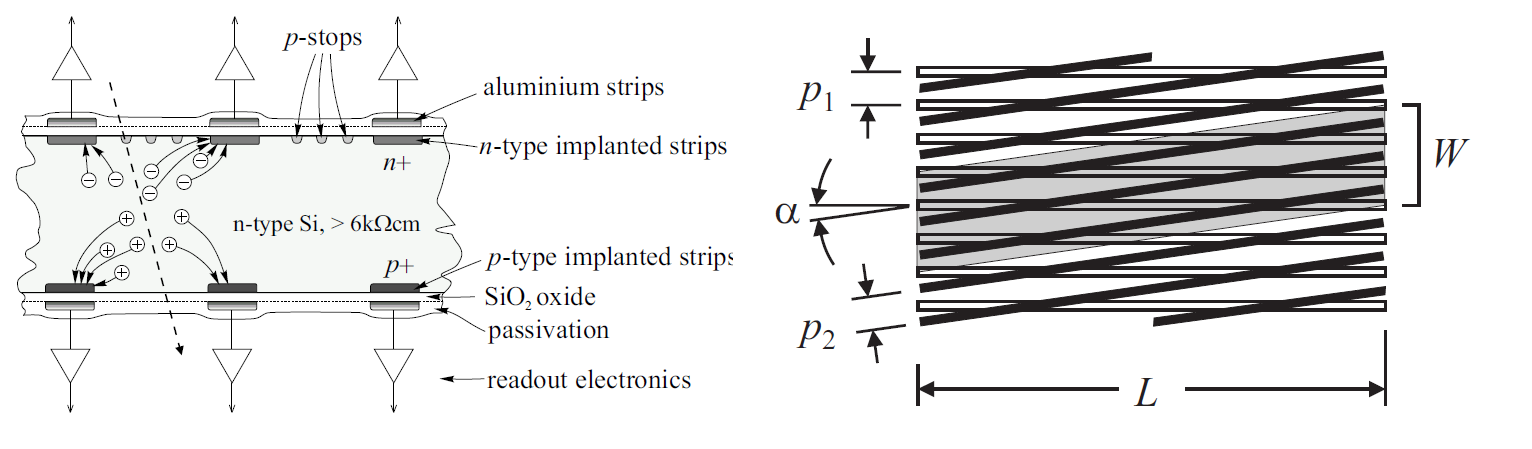
\includegraphics[width=1\columnwidth]{Chapter2/images/silicons.png}
\caption{The segmented electrode enables defining the particle position (left)~\cite{Sokolov:2006vdx}. The right scheme depicts the strips oriented at a small angle, which aims to reduce fake hits~\cite{Spieler}.}
\label{fig_si}
\end{figure}
\newpage


The sensitive volume of a silicon sensor produces the average signal current given by 
\begin{equation}
    Q_{s} = \frac{E}{E_{i}}e
\end{equation}
where E is the absorbed energy, $E_{i}$ is the energy required to form a charge pair. The energy needs to be greater than the bandgap, so that the electron can move to the conduction band. The silicon has a gap of 1.12~eV. Nevertheless, the commonly used ionization energy for silicon is about 3.6~eV. This effect is related to the fact that only about 30\% of the particle's energy is converted into electrical signal, the rest goes into phonon excitation.



\section{Radiation damage to the silicon sensors} 

The most important formula which allows for the trackers to be used in particle physics is Bethe-Bloch formula:

\begin{equation}
-\dfrac{\mathrm dE}{\mathrm dx} = 4 \pi N_{a} r_{e}^{2} m_{e} c^{2} z^{2}  \dfrac{Z}{A} \frac{1}{\beta^{2}} \left[ \frac{1}{2}\ln(\frac{2m_{e}\gamma^{2}c^{2} T_{max}}{I^{2}}) - \beta^{2} -  2\frac{\delta(\gamma)}{Z}\right]
\end{equation}

Where z is the charge of the particle, $T_{max}$ is the maximum kinetic energy that can be imparted to a free electron in a single collision, I is the mean excitation energy, Z the atomic number, A the atomic mass, $N_{A}$ the Avogadro’s number, $m_{e}$ the electron mass, c the speed of light, $r_{e}$ the classical electron radius, $\beta = v/c$ and $\gamma = \frac{1}{\sqrt{1-\square\beta}}$ and $\delta$ density effect correction. It describes the average energy loss of a charged particle in a given medium (for example, gas or a semiconductor). 

Radiation damage can be divided into two main groups: displacement damage and ionization damage. The first mentioned phenomenon is related to the incident particles displacing the silicon atoms from their position in the lattice. The ionization damage occurs in the insulating layers of the sensor. 

The influence of the radiation on the silicon is described by so-called Hamburg model. 

The traversing particles are not only causing the ionization of the lattice, but also interact with the silicon via electromagnetic and strong forces. Atoms can be displaced and create defects. Those defects populate new levels in the band gap, changing the properties of the silicon. That’s why the performance of the silicon sensor will degrade over time, what should also be considered while designing an experiment. The leakage current of a sensor after irradiation is related to the fluence as follows:
\begin{equation}
\label{eq:fluence}
    I_{d} = I_{0} + \alpha + \phi + Ad
\end{equation}
where $I_{0}$ is the leakage current before the irradiation, $\alpha$ is a damage coefficient dependent on particle type and temperature, $\phi$ is the particle fluence, d is the detector thickness, and A is the area. 
Typical values for the damage coefficeint reach 


\begin{equation}
\label{Sil:temp}
    I_{R}(T) \propto T^{2}e^{\frac{-E}{2kT}}
\end{equation}
 By assuming that one of the  temperature sensors at a similar height as the silicon sensors mimics their temperature. This assumption clearly doesn't consider several effects like silicon sensors' self-heating. Nevertheless, it allows us to scale down leakage current to $20\,^{\circ}$C using the equation \ref{Sil:scal}.
 
\begin{equation}
\label{Sil:scal}
    \frac{I_{R}(T_{2})}{I_{R}(T_{1})} = (\frac{T_{2}}{T_{1}})^{2}e^{\frac{-E}{2kT}\frac{T_{1}-T_{2}}{T_{1}T_{2}}}
\end{equation}

\begin{figure}[!h]
\centering
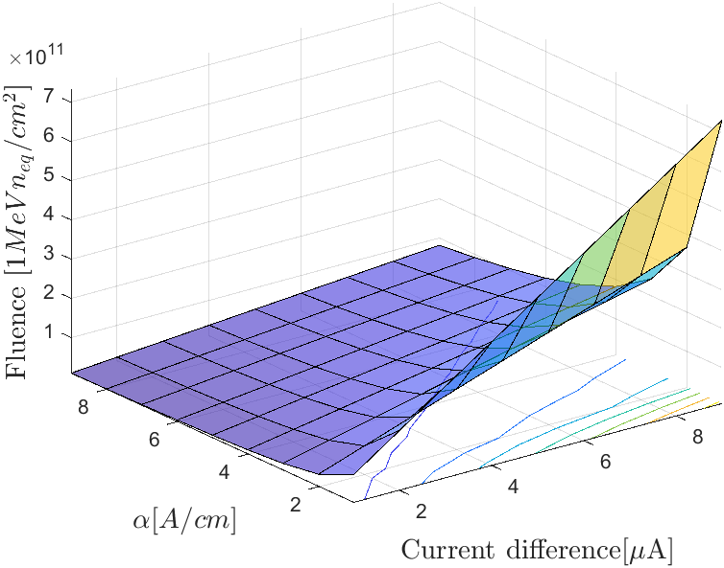
\includegraphics[width=0.65\columnwidth]{Chapter2/images/Leakage_current.png}
\caption{Fluence estimations based on the equation~\ref{eq:fluence} for the typical leakage changes during the \gls{mCBM} experiment.}
\label{fig_leakage}
\end{figure}

\begin{figure}[!h]
\centering
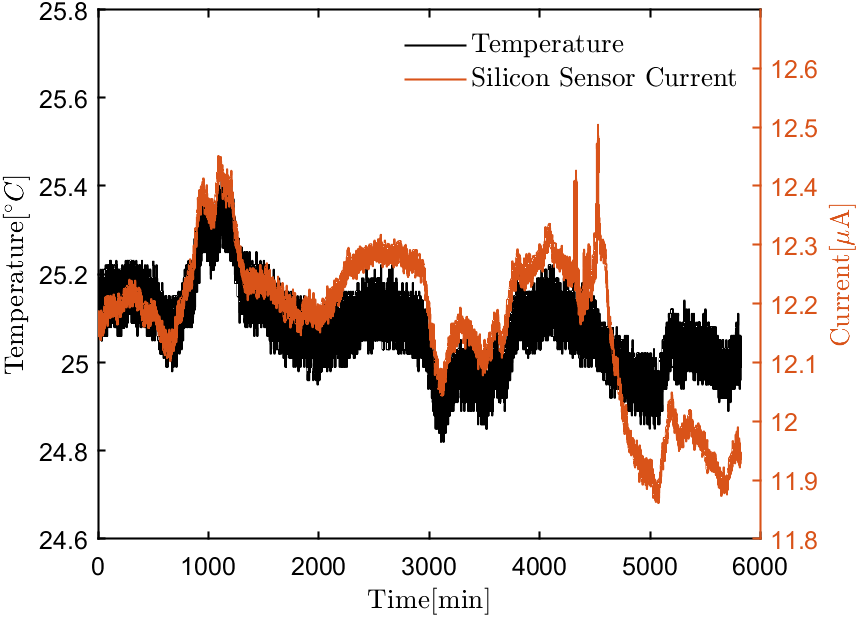
\includegraphics[width=0.65\columnwidth]{Chapter2/images/currenttempnobeam.png}
\caption{The first proposition of the CBM readout chain based on separate DPB and FLIB boards \cite{CRI}}
\label{fig_leakage1}
\end{figure}




\section{Design of STS}
\label{STS}

The physics observables together with the foreseen accelerator specifications mentioned in the previous chapter define the requirements for the detector system. The \gls{STS} is designed to provide track reconstruction and momentum determination of the charged particles. The detector has to work with ion beam energies from 2 to 14 AGeV (protons 39 GeV). In addition to that, a very high interaction rate 10~MHz results in up to 700 tracks per central Au+Au collisions. The \gls{STS} extends more than \SI{1}{\metre} downstream of the target and will be installed in a volume of \SI{3}{\square\metre}. 

In order to achieve physics goals, \gls{STS} has to address the following:
\begin{itemize}
    \item  aperture - the aperture of the whole experiment is expected to cover polar angles from \SI{2}{\degree} up to \SI{25}{\degree}. This range corresponds to center-of-mass rapidity close to the beam rapidity. 
    \item spatial resolution - a single-hit resolution of about \SI{20}{\micro\metre} in X direction and \SI{120}{\micro\metre} in Y, 
    \item single-hit efficiency - the detector layer should provide almost 100\% detection efficiency. The damaging effect of the radiation, implies that the \footnote{ratio of the most probable amplitude for a minimum ionizing particle divided by the root mean square of the single strip noise}{signal-to-noise} ratio needs to be over 10. Having that, the track reconstruction efficiency should exceed 95\% for particle momenta larger than 1~GeV/c. 
    \item momentum resolution - it's mainly influenced by the material budget of the system. The \gls{STS} is designed with the aim to avoid excessive multiple scattering. It is achieved by placing the electronics, mechanical infrastructure and cooling outside the active area. For the \gls{STS} the momentum resolution of $\Delta p/p = 1.5\%$ is foreseen. 
    \item radiation hardness - the silicon sensors and the electronics need to withstand the total dose of 10~kGy~\cite{Heuser:54798}. It was confirmed that after receiving twice the mentioned dose the charge collection efficiency decreases by up to 20\%. 
    \item hit rates and readout - the hit rates of charged particles for the inner-most silicon sensors (10~MHz per $\mathrm{cm^{2}}$ provide the requirements for the readout system (signal shaping time, number of readout channels etc.)
\end{itemize}

A simplified CAD drawing of the \gls{STS} is presented in Figure~\ref{fig_STS}. 

\begin{figure}[!h]
\centering
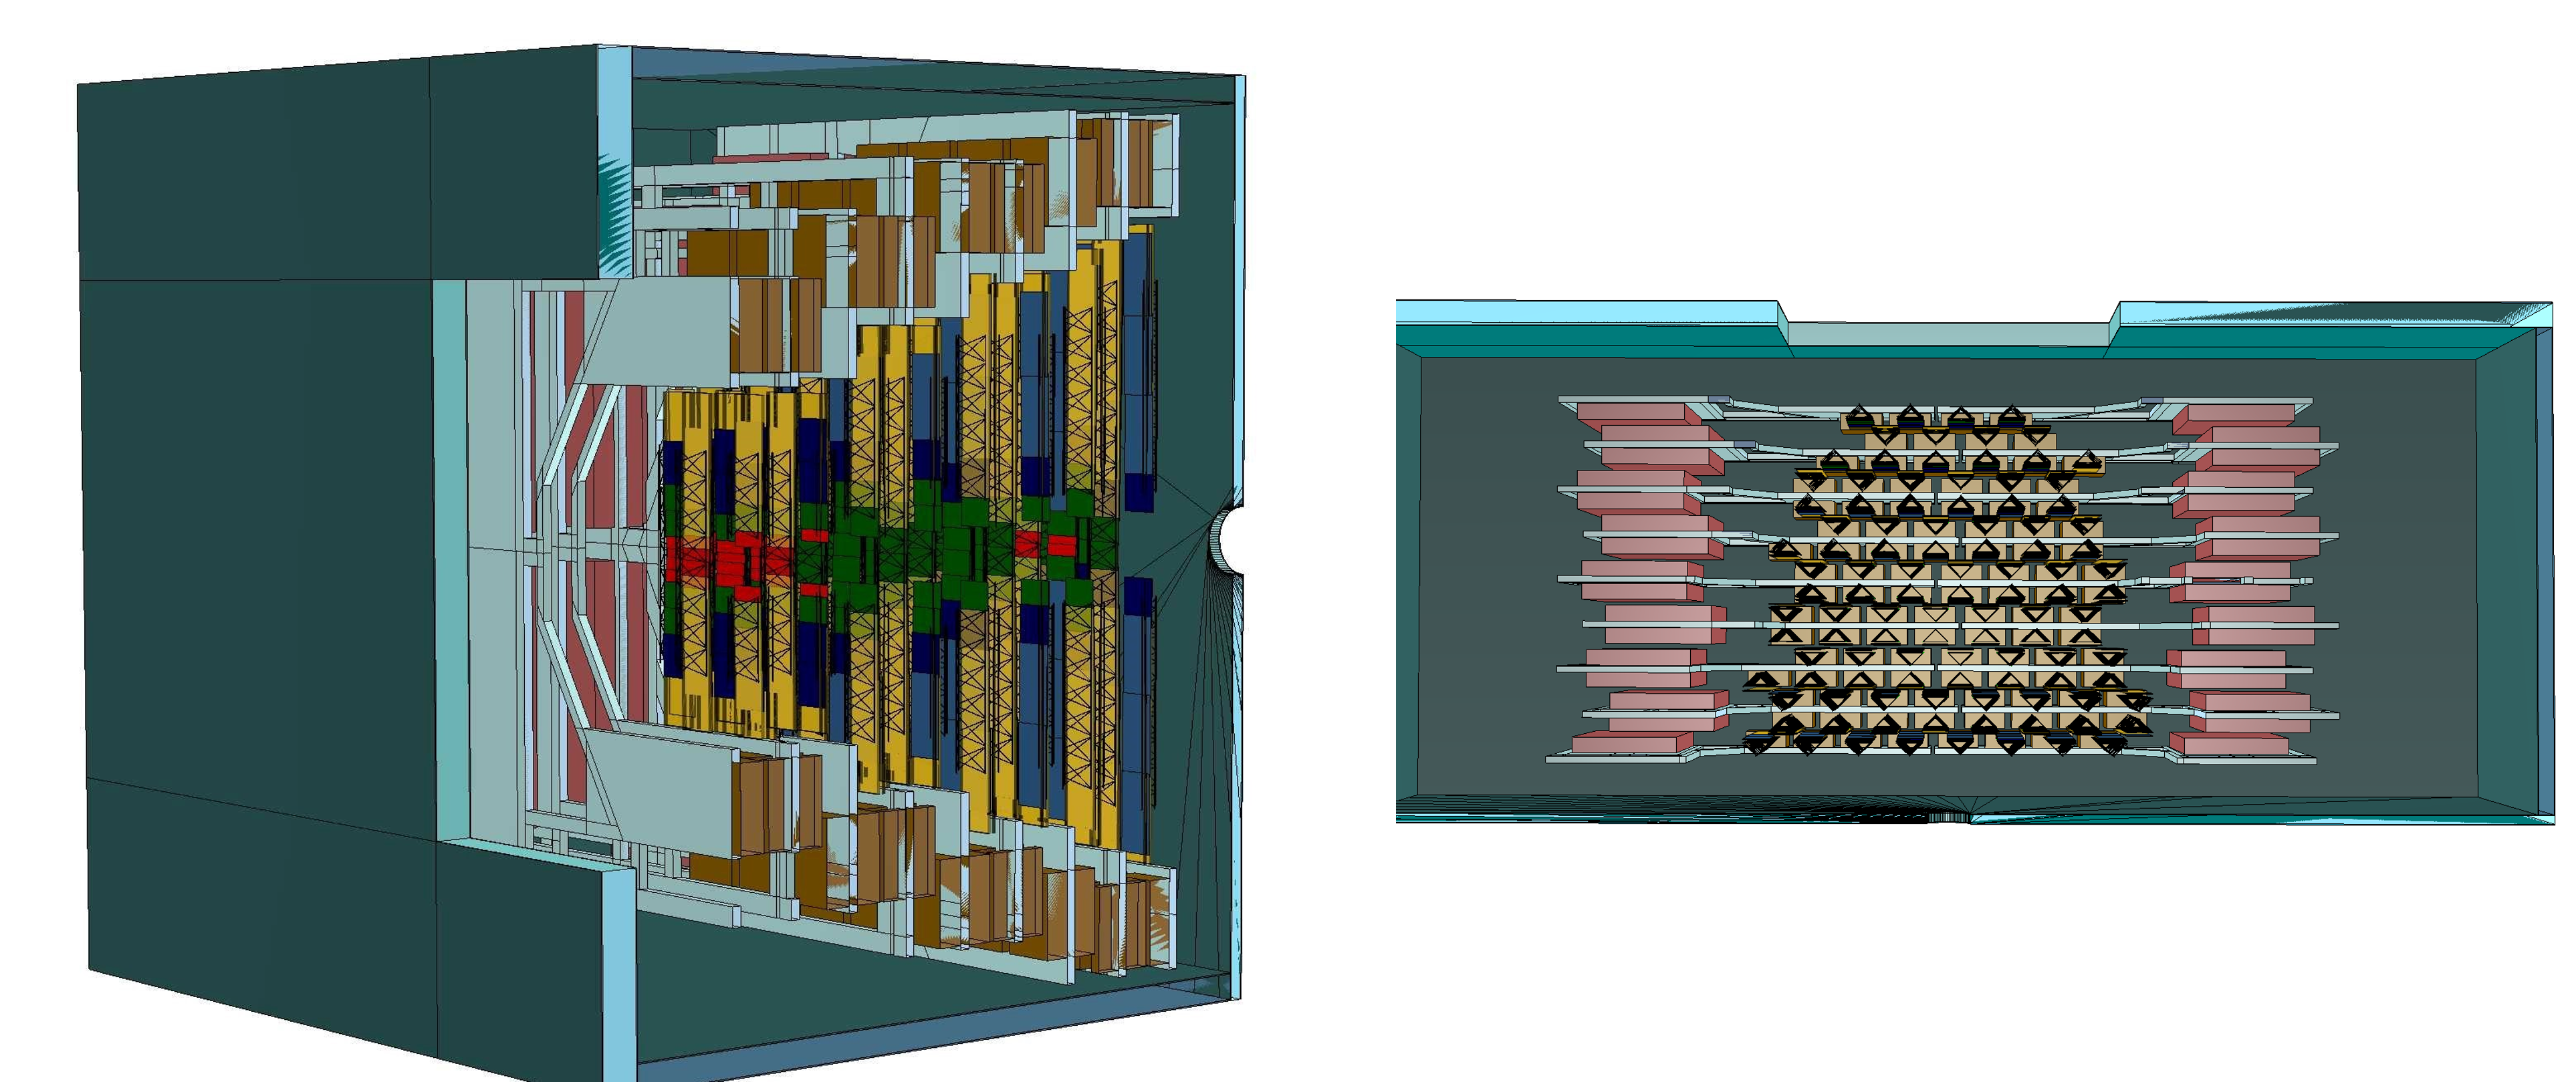
\includegraphics[width=0.85\columnwidth]{Chapter2/images/STS.png}
\caption{A simplified geometry of the Silicon Tracking System. The 8 tracking stations cover the polar angle from \SI{2}{\degree} up to \SI{25}{\degree}.}
\label{fig_STS}
\end{figure}

The detector consists of 876 detectors modules. A module is composed of double-sided silicon microstrip sensors, ultralight microcables (of up to 50~cm length) and Front End Boards (\gls{FEB}) populated with ASICs (STS-XYTER) glued on the fins. The modules are distributed on carbon fiber support-structures which populate C-frames~\cite{progress_report_2016}. Two C-frames form a tracking station of \gls{STS}.  Figure~\ref{fig_assembly} depicts a simplified assembly workflow of \gls{STS}.
The modules are produced in 166 variants, which differ in sensors size, micro-cable length and the orientation of the Front End Electronics~(\gls{FEE}).  


The stations are placed inside a thermally insulated box which resides in a dipole magnet. During \gls{STS} operation, the temperature inside the enclosure will be gradually decreased with the increasing radiation damage to the silicon sensors, to ensure no risk of thermal runaway~\cite{Spieler}. In principle, the largest amount of heat is dissipated by the low-voltage powering of the electronics and not the sensors themselves. Hence, an effective cooling is needed to address this problem.
The temperature of about \SI{-10}{\celsius} will ensure a safe performance of the semiconductors and minimize the contribution of the shot noise~\cite{Spieler}. The low ambient temperature also sets hard limits on the frost point. As the coolant temperatures might reach down to \SI{-40}{\celsius}, the frost point needs to be below \SI{-45} at all times. 

\newpage
\begin{figure}[!h]
\centering
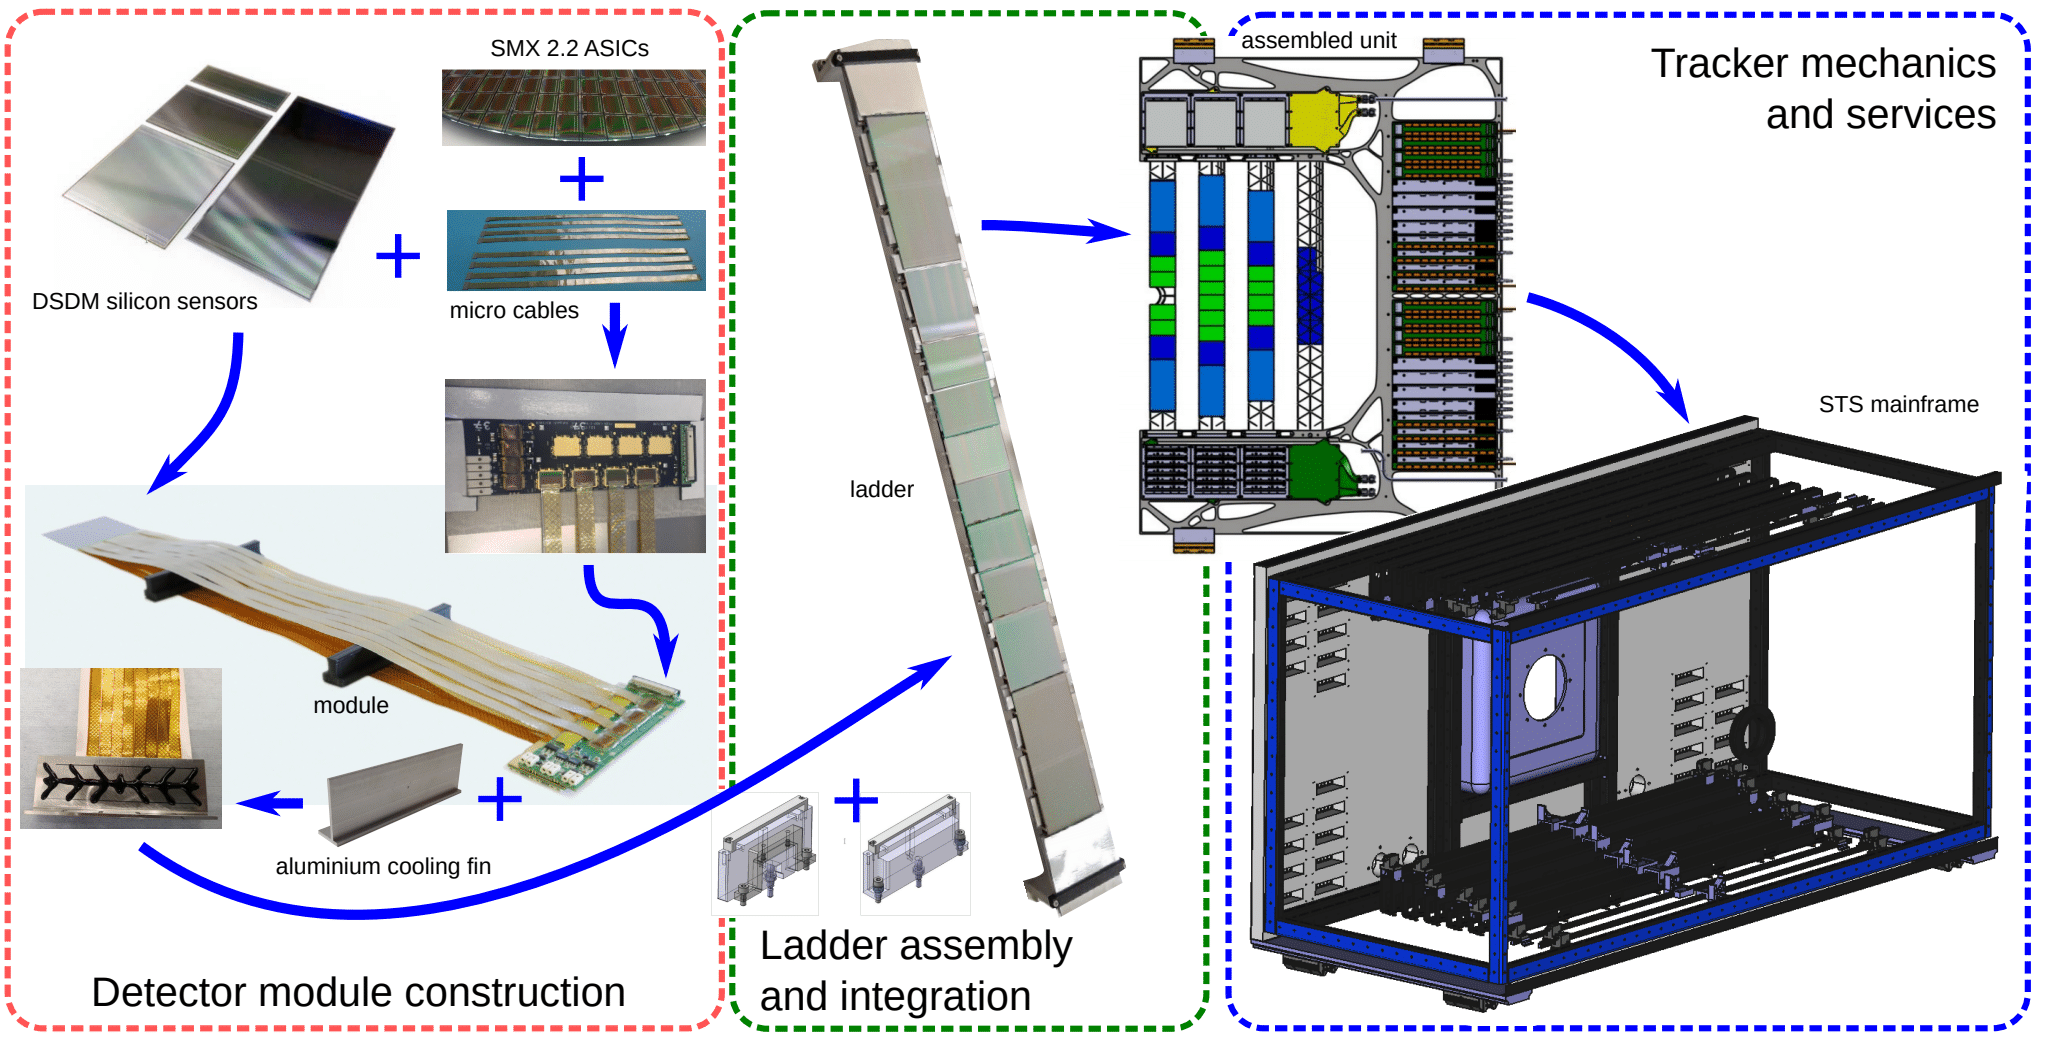
\includegraphics[width=1\columnwidth]{Chapter2/images/assembly_sequence.png}
\caption{A simplified assembly workflow of the \gls{STS}. The silicon sensors are connected to the ASICs on the \glspl{FEB} via microcables. The modules are assembled into carbon fiber ladders which form a C-frame. (Private information from M. Teklishyn)}
\label{fig_assembly}
\end{figure}

%The evolution of different experimental setups constructed for the purpose of testing components of the \gls{STS} is depicted in Figure \ref{fig_evolution_STS}. 

%\begin{figure}[!h]
%\centering
%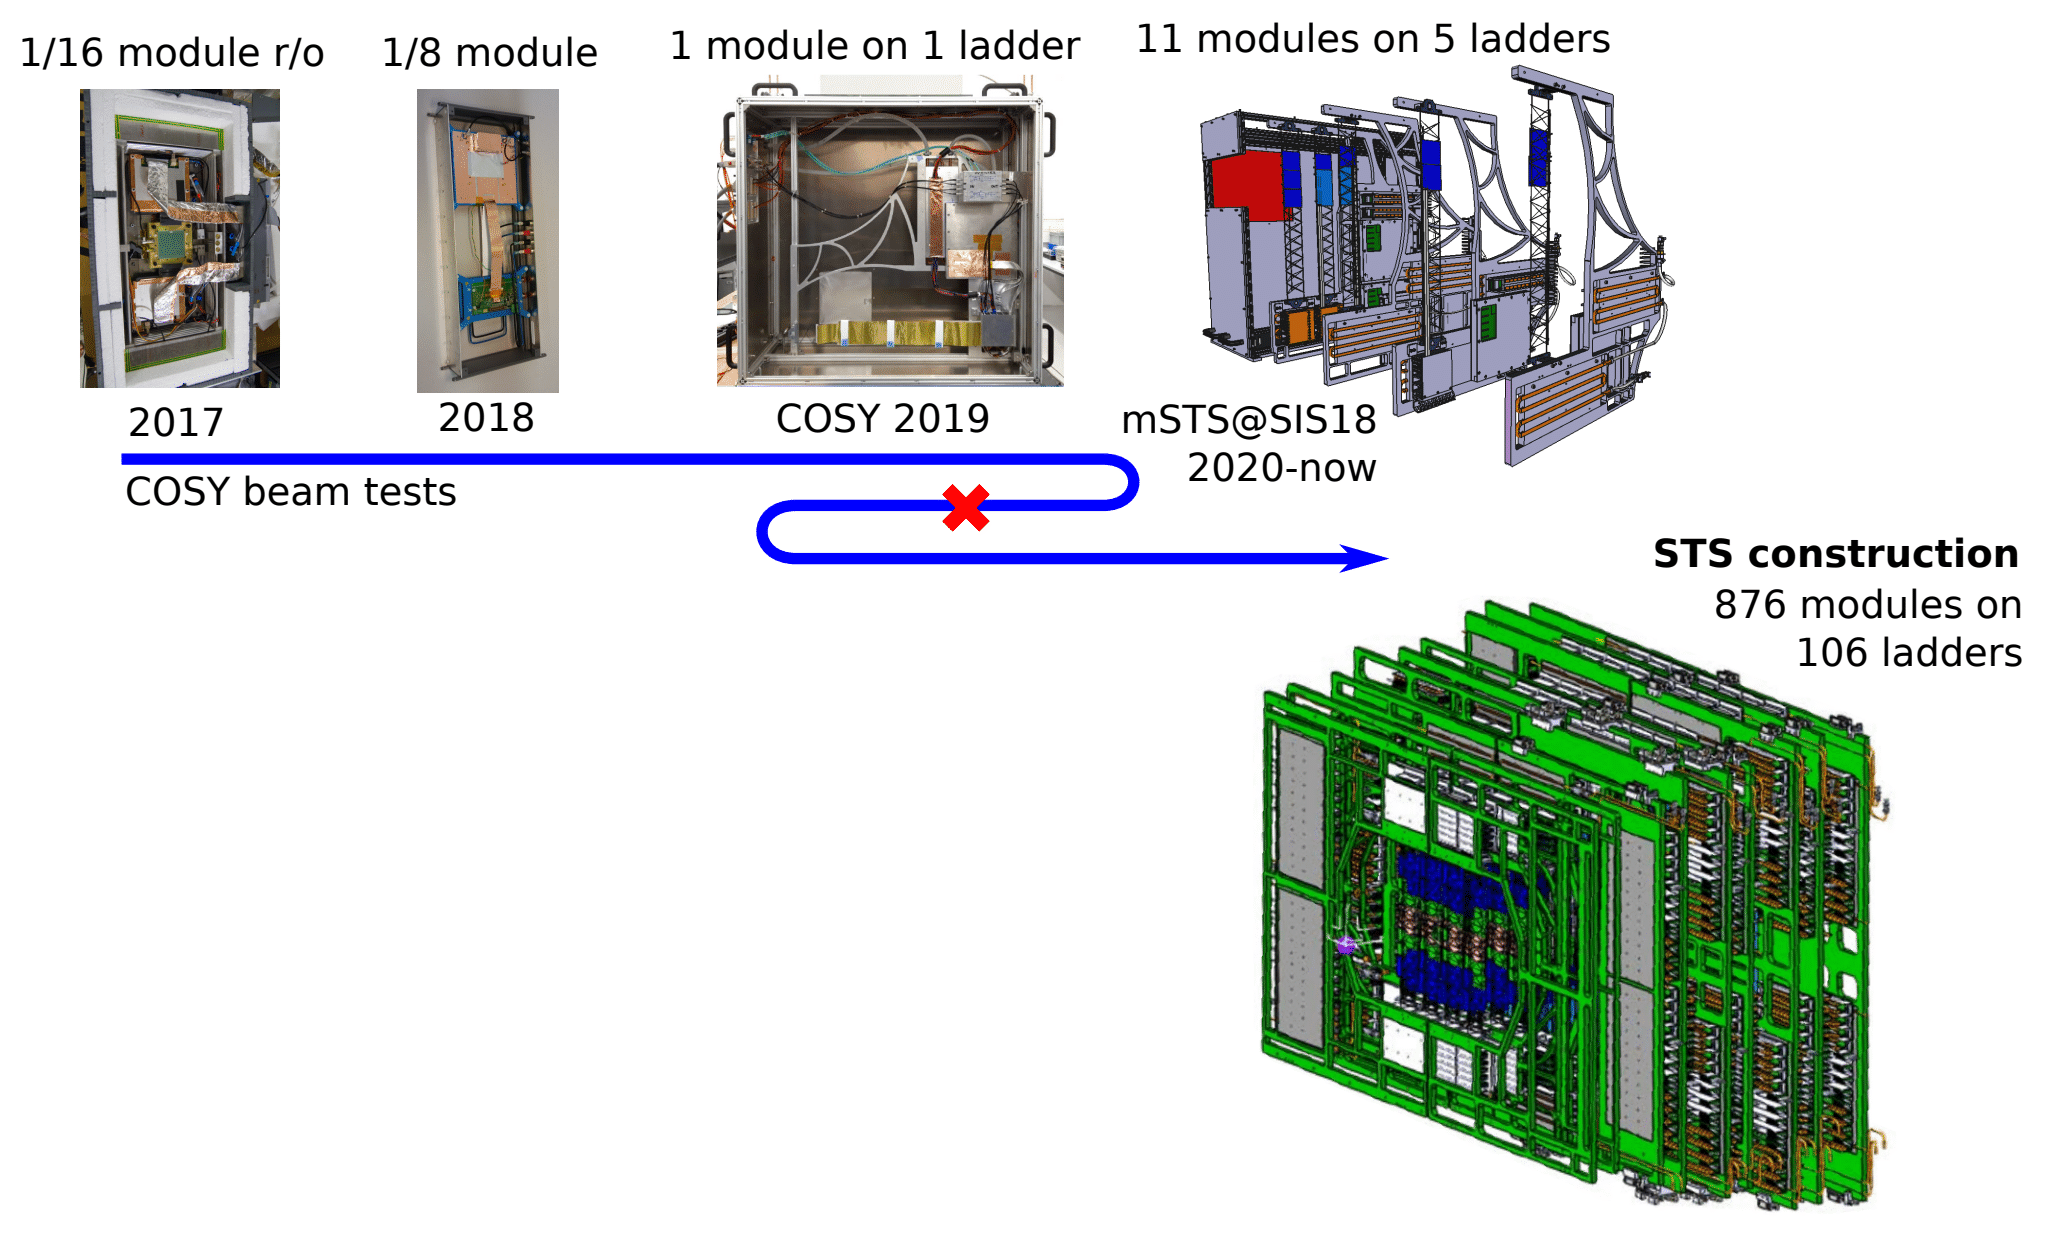
\includegraphics[width=0.95\columnwidth]{Chapter2/images/evolution_sts_new.png}
%\caption{Evolution of the test setups towards \gls{STS}. (Private information %from M. Teklishyn)}
%\label{fig_evolution_STS}
%\end{figure}




\subsection{Double-sided microstrip silicon sensors}
\label{sensors}

The use of microstrip silicon sensors has been demonstrated in many well-known experiments like those operated at \gls{CERN}(\gls{ALICE} and \gls{CMS}) and Brookhaven National Laboratory (\gls{STAR}). The aluminum strips on the p-side of the sensors are inclined by \SI{7.5}{\degree} with respect to the n-side. That implies that there is a set of shorter strips on the p-side. These strips are interconnected with each other using a second metallization layer on the sensors. An example of this solution is presented in Figure~\ref{fig_sts_si}. 

\begin{figure}[!h]
\centering
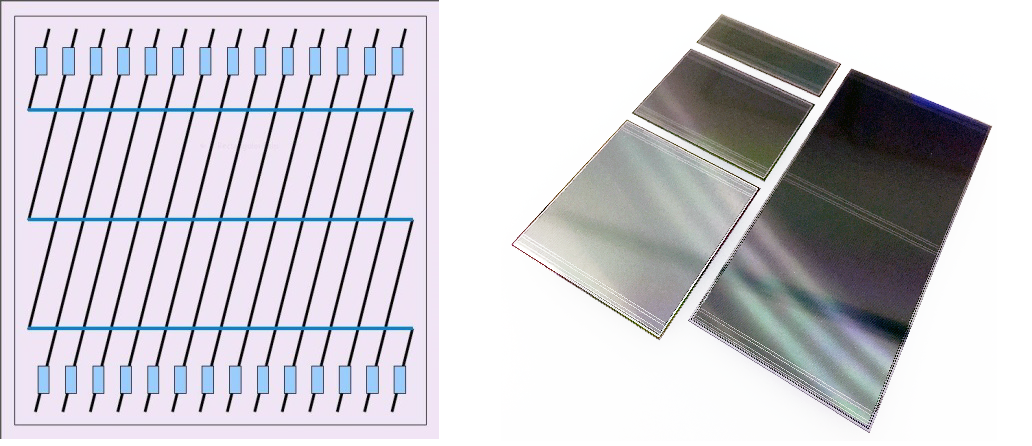
\includegraphics[width=0.75\columnwidth]{Chapter2/images/silicon_sensors.png}
\caption{Left: An example of sensor's electrode segmented into strips inclined by a small angle. The shortest strips are interconnected with each other. Right: The silicon sensors to be used for the \gls{STS}. The width of the sensor is \SI{6.2}{\centi\metre} and there are 4 strip lengths: \SI{2.2}{\centi\metre}, \SI{4.2}{\centi\metre}, \SI{6.2}{\centi\metre}, \SI{12.4}{\centi\metre}.}
\label{fig_sts_si}
\end{figure}

The sensors are produced on \SI{320}{\micro\metre} thick n-type wafers by Hamamatsu Photonics K.K. Each of the sensors features 1024 strips with \SI{58}{\micro\metre} pitch. The signal from the sensors is transported to the front-end electronics via ultra-light microcables. These cables are additionally shielded to protect the analog signals from any interference. 

\subsection{Module}
\label{module}
 The assembly of the detector is realized stepwise. The whole complex procedure requires utmost care and extremely high precision. Therefore, a proper workflow was developed to address the complexity of the module assembly~\cite{carmen2}.

\section{The readout chain of the STS}
\label{readout}
\label{DAQ}
The \gls{STS} readout chain is designed to control, readout and preprocess analog signals acquired from the silicon sensors. Moreover, it has to handle a high data throughput and store it. The \gls{CBM} experiment is going to run with a free-streaming Data Acquisition (\gls{DAQ}) system. It is made of the \gls{FEE}, data transport, online event reconstruction and online event selection~\cite{Kasinski1}.

The first layer of the \gls{STS}'s readout chain consists of Front-End Board (\gls{FEB}) which is populated with 8  Application-specific integrated circuits (ASICs)~\cite{Kasinski2}. Each ASIC or STS-XYTER is responsible for readout of 128 channels. The chips feature the analog front-end (\gls{AFE}), the digitizer and generation of hits using Analog Digital Converter (\gls{ADC}) and timestamp information. 

The next element, which transports data from the \gls{FEE} is the readout board (\gls{ROB}). It aggregates data from multiple \glspl{FEB} and sends it via optical links out of the detector enclosure to the Common Readout Interface (\gls{CRI}) board. Subsequently, the data is transported to the First Event Level Selector (\gls{FLES}). 
\newpage
In total, the \gls{STS} features roughly, 14000 STS-XYTERs, 600 \glspl{ROB}. Given a typical average raw event size of roughly 50 kB for minimum-bias Au+Au collisions, a peak collision rate of 10~MHz results in an instantaneous raw data rate of about 500~GB/s (for the all the detector systems).

\begin{figure}[!h]
\centering
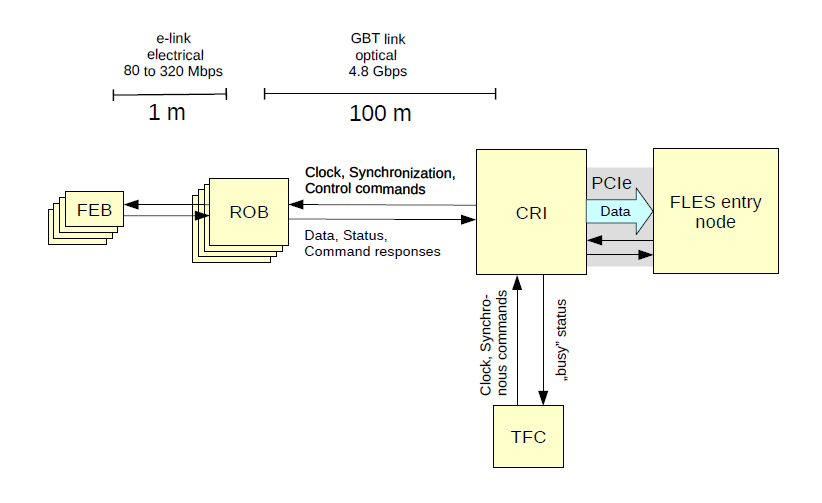
\includegraphics[width=0.8\columnwidth]{Chapter2/images/CRI_DAQ.png}
\caption{The basic building parts for one \gls{FLES} entry node are shown schematically. An entry node can hold many \glspl{CRI}. A \gls{CRI} often serves numerous \glspl{ROB}, whereas a \gls{ROB} typically serves multiple \glspl{FEB}. The Timing and Fast Control (\gls{TFC}) is a core system that is shared by all \glspl{CRI}.}
\label{fig_daq_cri}
\end{figure}

There are two other readout chains that have been exercised for different detector development activities. The first option is based on Data Processing Board (\gls{DPB}).
The second option is the readout chain based on the  GBTxEMU-based tester, which emulates the \gls{ROB}.


\subsection{Front-end electronics (FEE) and the readout ASIC}

A readout of a detector module is based on the two \glspl{FEB} (see Figure~\ref{fig_feb}) which has 8 STS-XYTERs each. These chips discriminate and digitize the analog signals coming through the microcables from the silicon strips. As described in the section \ref{STS}, the \glspl{FEB} are located in the perimeter of the detector stations and will receive up to 100krad/year~\cite{Heuser:54798}.

\begin{figure}[!h]
\centering
\includegraphics[width=0.45\columnwidth]{Chapter2/images/feb_8_v2.pdf}
\caption{Prototype design of a \gls{FEB} for reading out 1024 channels from the silicon sensors. There are 8 readout ASICs and four low dropout voltage regulators on the left. These active parts are covered in a protective glue called glob top.}
\label{fig_feb}
\end{figure}

The data load for the sensors will vary depending on the position in the detector. Each readout link of the \gls{FEB} has a bandwidth of about 320 Mb/s, therefore for the innermost sensors the \gls{FEB} has 5 readout link instead of 2 or 1. 

The dimensions of the \gls{FEB} are tightly constrained due to the limited space inside the \gls{STS}. Hence, the dimensions of the \gls{FEB} are approximately \SI{3}{\centi\metre} by \SI{10}{\centi\metre}. The chips need also to be powered, what is achieved by the linear voltage regulators (\gls{LDO} regulators). Each \gls{ASIC} has an analog (VDDM) and digital power domain that are powered by 1.2~V and 1.8~V \glspl{LDO}. The analog part is powered by 1.2~V and 1.8~V \glspl{LDO}, whereas the digital part is supplied from 1.8~V \gls{LDO}.

\glspl{FEB} are glued to aluminum fins, in order to achieve good thermal coupling. Subsequently, the fins are fixed to the base plate of the \gls{FEB} box (see Figure~\ref{feb_box}) before mounting them on a ladder. The \gls{FEB} boxes reside on cooling plates. The carbon composite has an ultrahigh thermal conductivity, therefore the excess heat is efficiently removed by the coolant (NOVEC 649) which circulates through the cooling plate providing temperature down to \SI{-40}{\degree}. 

\begin{figure}[!h]
\centering
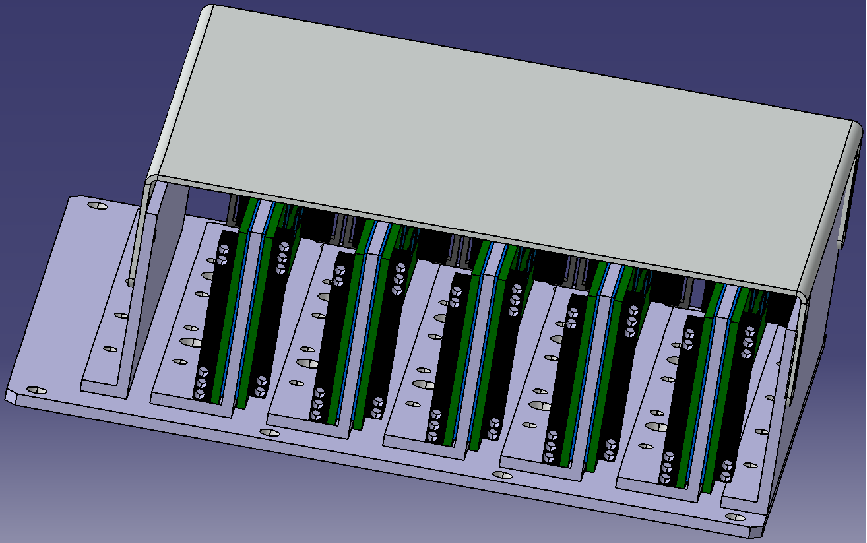
\includegraphics[width=0.45\columnwidth]{Chapter2/images/feb_box.png}
\caption{A simplified CAD drawing of the \gls{FEB} box.}
\label{feb_box}
\end{figure}


The characterization of the STS-XYTER ASICs is an extensive procedure which investigates the chip. Information about proper amplitude and time calibrations are necessary to interpret the data correctly. This represents an essential step before using the chip in the readout of the silicon sensors. The characterization procedures are intended to
check many parameters that influence the \gls{FEB} performance. 


\subsubsection{Design of the STS-XYTER}

The STS-XYTER (see Figure~\ref{sts_xyter}) is an integrated circuit designed for the readout of \gls{STS} and \gls{MUCH} consisting of 128 analog channels. Those channels are connected to the silicon sensors via silicon sensors. One of the elements of the chip is a so-called low noise charge sensitive amplifier (\gls{CSA}), which converts the aggregated charge into a voltage step with amplitude proportional to the charge. Subsequently, the signals pass through the polarity selection circuit (\gls{PSC}) which assures that a single polarity prevails. It makes the use of a double-sided silicon sensors feasible. The signal processing is distinguished into two paths: fast and slow. The first one is responsible for the determination of the timestamp and the second one has been adjusted for low noise discrimination and energy measurement with a 5-bit flash ADC. When operating the \gls{ASIC} in self-triggered mode, hit information is saved and latched by the arrival of each signal using the information from the 5-bit continuous-time ADC and two mentioned paths. 

\begin{figure}[!h]
\centering
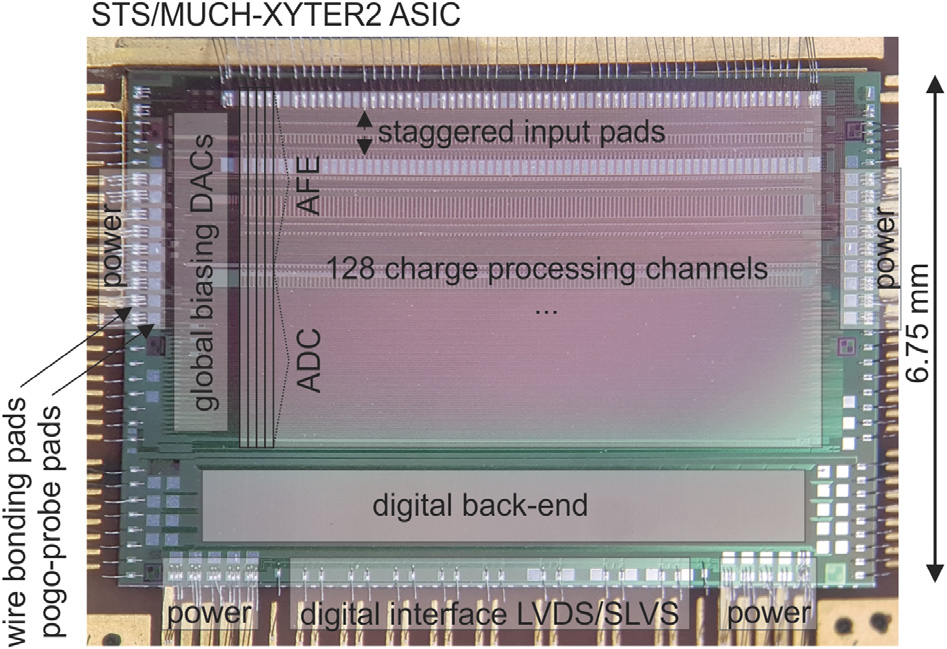
\includegraphics[width=0.65\columnwidth]{Chapter2/images/ASIC2.2.png}
\caption{The final version of the STS-XYTER chip with the major parts marked~\cite{KASINSKI2018225}.}
\label{sts_xyter}
\end{figure}

The digital back-end allows for register access and data readout. It also provides measures to monitor the performance of the chip via i.e., upset counters, link error monitor, diagnostic circuitry (temperature, VDDM potential, CSA bias value). The communication with the chip is based on a custom developed Hit and Control Transfer Synchronous Protocol (STS-HCTSP) protocol~\cite{Kasinski_2016}. A detailed description of the STS-XYTER can be found in the PhD thesis of A. Rodriguez~\cite{RodriguezRodriguez2020}.

STS-XYTER also features an internal monitoring circuit - diagnostic circuit. It enables measurement of several potentials inside the chip. By monitoring the analog powering domain (VDDM), temperature it's possible to have a general understanding of the chip state without running extensive tests. The diagnostic circuit of the \glspl{ASIC} and the obtained results will be discussed in detail in Chapter 4.

\subsection{Readout board (ROB) and Common Readout Interface (CRI)}

The \gls{STS} readout board is a data concentrator board based on the radiation-tolerant GBTx ASIC and Versatile Link
devices developed by CERN and others~\cite{Bonacini:1235849, C_2013}. The board is an interface between many electrical readout links (many \glspl{FEB}) and the \glspl{CRI} boards located outside the underground cavern of the \gls{CBM} experiment~\cite{Lehnert_2017}. It resides inside the \gls{STS} enclosure, what means that it will be exposed to high radiation levels. Therefore, it's built from radiation hard components. The board is also thermally coupled to the cooling plate, which can reach temperature down to \SI{-40}{\degree}. The \gls{ROB} needs to reliably work at changing temperature between \SI{-40}{\degree} and \SI{20}{\degree}. 

The main building elements of the board are three \gls{GBT}x \glspl{ASIC} and a \gls{GBT} \gls{SCA2} \gls{ASIC}. Two of the \glspl{GBT}x \glspl{ASIC} act as slaves and are controlled via the mentioned \gls{SCA2}. 

The Common Readout Interface (\gls{CRI}) is a \footnote{PCIe card refers to a kind of network adapter with a PCIe interface.}{PCIe card} based on Field Programmable Gate Arrays (\gls{FPGA}). The \gls{CRI} provides the input to the First-level Event Selector (\gls{FLES}). It's also a central element of the \gls{DAQ} chain, as it provides means of data control. Moreover, the \gls{CRI} has interface to the \gls{TFC} system. 
\begin{figure}[!h]
\centering
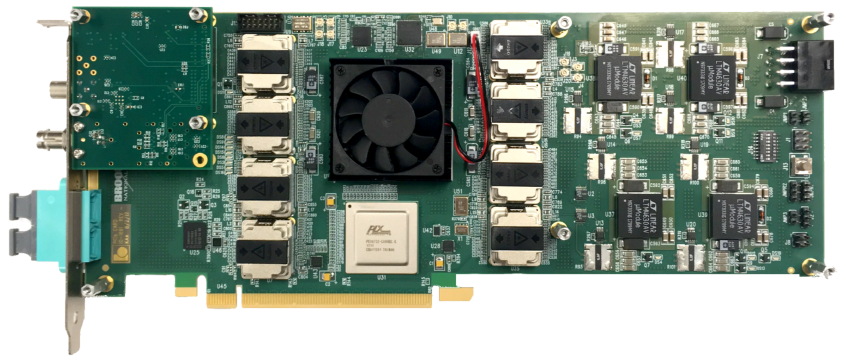
\includegraphics[width=0.7\columnwidth]{Chapter2/images/cri_board_atlas.pdf}
\caption{The first prototype of the \gls{CRI} board~\cite{CRI}.}
\label{fig_cri_board}
\end{figure}


\subsection{Alternative readout chains}
\label{tester}
There are two alternative readout chains implemented for the testing purposes towards realization of \gls{STS}. The first readout chain is based on the Data Processing Board (\gls{DPB} is a \gls{FPGA} based board), \glspl{ROB} and the second one features GBTxEMU-based.\bigbreak


\textbf{DBP based chain}\bigbreak


Even though the final solution for the readout is the \gls{CRI} board, the Data Processing
Boards (\glspl{DPB}) were implemented for developing and testing purposes~\cite{Loizeau}. For the control communication with the \gls{DPB}, the IPbus protocol~\cite{ipbus} was chosen. It is a communication protocol based on Gigabit Ethernet (GbE) which allows a simple and fast communication with \glspl{FPGA}.\bigbreak

\textbf{GBTxEMU} \bigbreak


Another alternative to the two readout chains is the so-called GBTxEMU-based tester. It is based on a commercial Artix-7 board (TE-0712, Trenz Electronics Gmbh), and allows emulating GBTX ASIC or the whole \gls{CROB}. Moreover, it could also be used in an autonomous mode with the addition of an adapter.


The whole examination process towards \gls{STS} will include testing of about 20000 ASICs, then 2000 FEBs (tested  multiple times during the assembly, e.g., after the ASIC wire bonding and after the micro-cable bonding), and eventually the full module. As a hardware platform offering good availability and reasonable production cost, the GBTx65 EMU~\cite{zabolotny1} board was chosen.

The software used for the operation of the emulator board is also based on the IPbus~\cite{ipbus} protocol to access registers and a class for writing and reading the chip's registers. 
The operation begins from the full synchronization of the STS-XYTER links. This process enables the communication with the chip, given no correct time-phase between data and clock and incoming data exists. The next step involves the configuration of the chip's registers (35496 bits for the AFE control are set). At the same time, the number of enabled up-links, the channel masking and the timestamp counter are set.  From this point on, any custom tests or calibration may proceed. For example, read and write register tests, readout of the VDDM potential values, chip's temperature etc. Moreover, to enable long-term testing, an interface to the control system's framework was implemented.


\section{Overview of the services for the STS}

The \gls{STS} will feature a number of services and sensors that need to be controlled, monitored and automatized in order to work efficiently during the operation of the detector. These services include:
\begin{enumerate}
    \item Low voltage and high voltage powering modules.\\
    About 2500 low voltage and 900 high voltage powering channels will be employed for the \gls{STS}. The crates featuring these powering modules will be located in the experiment cave. This location exposes the electronics to an elevated radiation levels. 
    \item Temperature, humidity, pressure sensors.\\
    A number of different sensors and technologies will be used to monitoring the ambient conditions inside the detector. Their performance and values are going to have a direct impact on the detector operation.
    \item Cooling plant.\\
    To avoid reverse annealing of the silicon sensors and thermal runaway scenarios, the detectors will be cooled with temperatures reaching \SI{-40}{\degree} at the end of its lifetime. The cooling plant providing the coolant is the crucial part of the safe operation of the detector.
    \item Air-drying system.\\
    The coldest points inside the \gls{STS} may reach temperatures down to \SI{-40}{\degree}. Therefore, the water content inside the enclosure has to be fairly below the coolant temperature to avoid possible icing or condensation on the electronics.
 \end{enumerate}

%\subsection{Powering schematics of the detector}
%\label{powering}
%\subsection{Cooling concept for the STS's electronics and %silicon sensors}
%\label{cooling}


\section{Requirements for the control system}
\label{sys:req}
Custom solutions that are applied in \gls{STS} make the control of this system very challenging. Different services imply different control solutions which need to be implemented.
A distributed control system should offer remote control, alarm detection, reporting and logging, modeling and simulation, data processing (archiving, retrieval, plotting, conversion, analysis), common time management, access security, and automatic \footnote{Sequencing, also known as sequential control, it controls the device in a pre-determined order.}{sequencing}.
In addition to that, the \gls{DCS} for the Silicon Tracking System (\gls{STS}) is being designed taking into consideration the following aspects:

 
 \begin{itemize}
    \item potential control framework should offer the possibility to control a variety of different services, which often have different communication protocols,
    \item logging, and monitoring - there should be reliable means of supervision of processes, containers, and \footnote{The input/output controller is a device that interfaces between an input or output device and the computer or hardware device}{Input/Output Controllers} (\glspl{IOC}).
    \item the control software should be horizontally and vertically scalable, when it comes to adding additional computing nodes or applications/Input Output Controllers (\glspl{IOC})/containers,
    \item supervision - it should be possible to integrate a sub-system oriented with higher-level control structures,
     \item flexible - applications should be easy to run on different operating systems and processor architectures,
     \item sustainability and support - the experiment is supposed to run for about 10 years, excluding the building and commissioning time. The control system should be sustainable and long-term support provided,
     \item reliability - the system should be highly available, minimizing the downtimes,
     \item network separation - it should be running in a dedicated network (divided into several service-oriented subnets) to have a good overview of the processes and communication between the nodes,
     \item \glspl{GUI} - all parameters/\footnote{In control theory, a process variable is the currently measured value of a particular part of a process which is being monitored or controlled}{process variables} should be available in a user-friendly Graphical User Interface (\gls{GUI}). In case of error or malfunction, it should be stated clearly by the software where the error happened, what could be the potential risk and what actions need to be taken.

 \end{itemize}
\newpage

